%%% Code for https://doi.org/10.6084/m9.figshare.17185718.v2

\documentclass[3mm]{standalone}

% Fonts
\usepackage{stix}

\usepackage{amsmath} % for tag in equations

\usepackage{xcolor}
\usepackage{graphicx}

\usepackage{tikz}
\usetikzlibrary{patterns}

\begin{document}

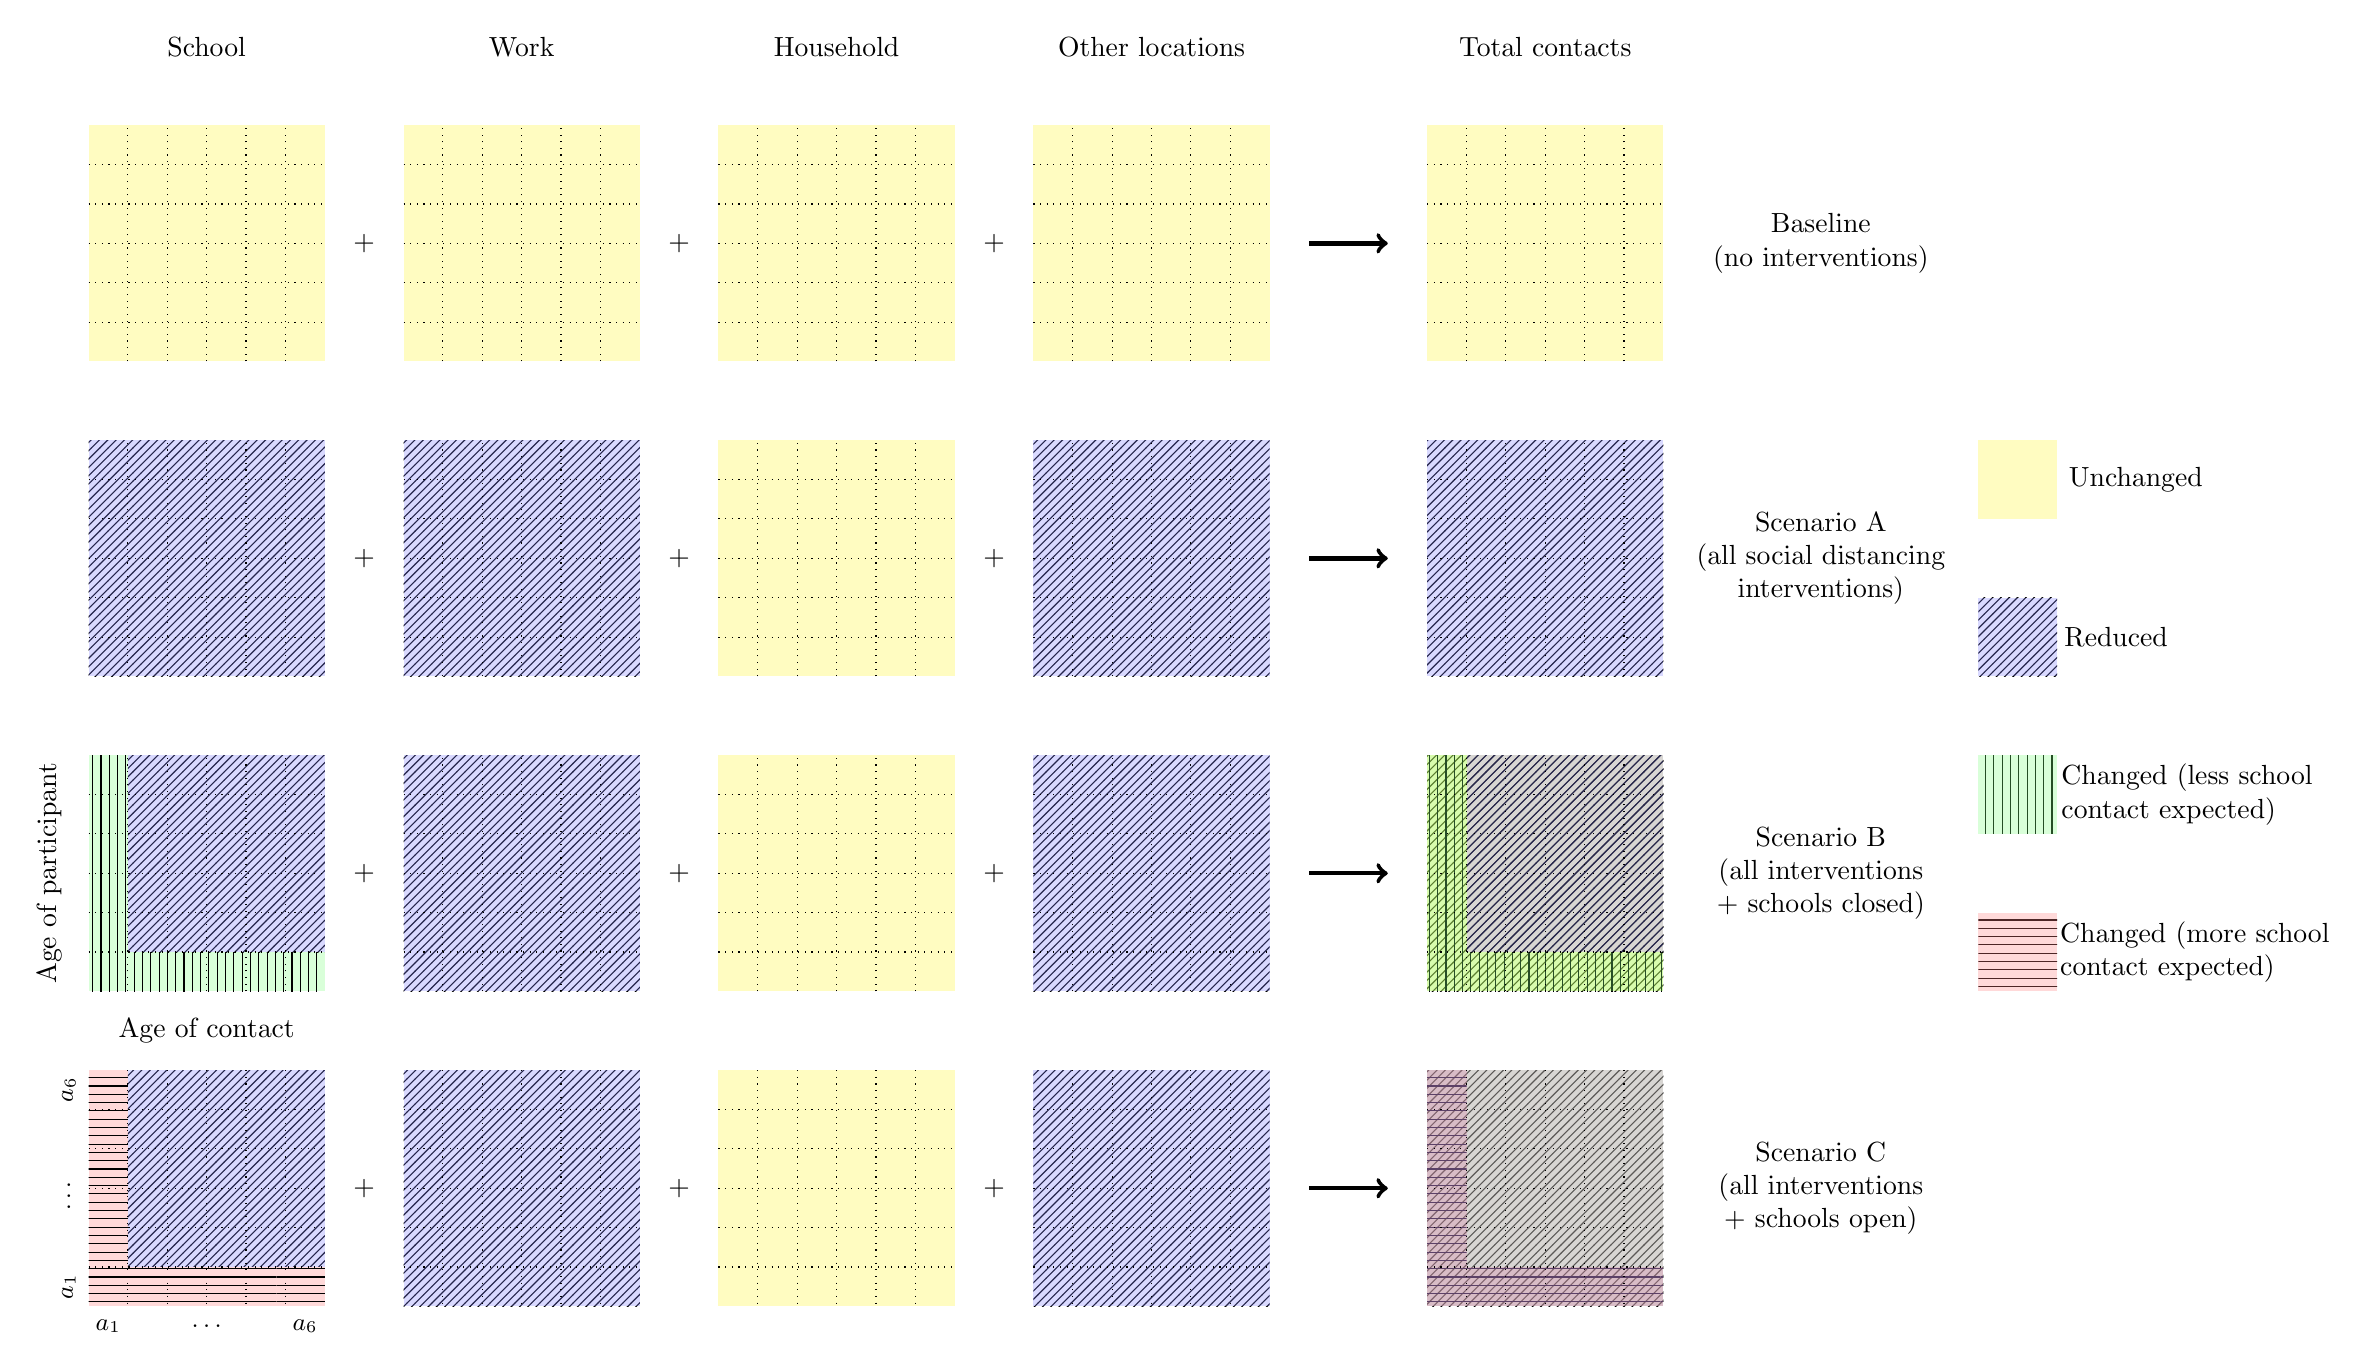
\begin{tikzpicture}
	% Top row
	\draw [draw = none, fill = white!20!yellow, fill opacity = 0.3] (0, 8) rectangle (3, 11);
	\draw [draw = none, fill = white!20!yellow, fill opacity = 0.3] (4, 8) rectangle (7, 11);
	\draw [draw = none, fill = white!20!yellow, fill opacity = 0.3] (8, 8) rectangle (11, 11);
	\draw [draw = none, fill = white!20!yellow, fill opacity = 0.3] (12, 8) rectangle (15, 11);

	% Second row
	\draw [draw = none, pattern = north east lines] (0, 4) rectangle (3, 7);
	\draw [draw = none, pattern = north east lines] (4, 4) rectangle (7, 7);
	\draw [draw = none, pattern = north east lines] (12, 4) rectangle (15, 7);
	
	\draw [draw = none, fill = white!50!blue, fill opacity = 0.3] (0, 4) rectangle (3, 7);
	\draw [draw = none, fill = white!50!blue, fill opacity = 0.3] (4, 4) rectangle (7, 7);
	\draw [draw = none, fill = white!20!yellow, fill opacity = 0.3] (8, 4) rectangle (11, 7);
	\draw [draw = none, fill = white!50!blue, fill opacity = 0.3] (12, 4) rectangle (15, 7);
	
	% Third row
	\draw [draw = none, pattern = north east lines] (4, 0) rectangle (7, 3);
	\draw [draw = none, pattern = north east lines] (12, 0) rectangle (15, 3);
	\draw [draw = none, fill = white!50!green, fill opacity = 0.3] (0, 0) rectangle (3, 0.5);
	\draw [draw = none, fill = white!50!green, fill opacity = 0.3] (0, 0.5) rectangle (0.5, 3);
	\draw [draw = none, pattern = vertical lines] (0, 0) rectangle (3, 0.5);
	\draw [draw = none, pattern = vertical lines] (0, 0.5) rectangle (0.5, 3);
	\draw [draw = none, pattern = north east lines] (0.5, 0.5) rectangle (3, 3);
	\draw [draw = none, fill = white!50!blue, fill opacity = 0.3] (0.5, 0.5) rectangle (3, 3);
	\draw [draw = none, fill = white!50!blue, fill opacity = 0.3] (4, 0) rectangle (7, 3);
	\draw [draw = none, fill = white!20!yellow, fill opacity = 0.3] (8, 0) rectangle (11, 3);
	\draw [draw = none, fill = white!50!blue, fill opacity = 0.3] (12, 0) rectangle (15, 3);

	% Fourth row
	\draw [draw = none, pattern = north east lines] (4, -1) rectangle (7, -4);
	\draw [draw = none, pattern = north east lines] (12, -1) rectangle (15, -4);
	
	\draw [draw = none, fill = white!50!red, fill opacity = 0.3] (0, -4) rectangle (3, -3.5);
	\draw [draw = none, fill = white!50!red, fill opacity = 0.3] (0, -3.5) rectangle (0.5, -1);
	\draw [draw = none, pattern = horizontal lines] (0, -4) rectangle (3, -3.5);
	\draw [draw = none, pattern = horizontal lines] (0, -3.5) rectangle (0.5, -1);
	\draw [draw = none, pattern = north east lines] (0.5, -3.5) rectangle (3, -1);
	\draw [draw = none, fill = white!50!blue, fill opacity = 0.3] (0.5, -3.5) rectangle (3, -1);
	\draw [draw = none, fill = white!50!blue, fill opacity = 0.3] (4, -1) rectangle (7, -4);
	\draw [draw = none, fill = white!20!yellow, fill opacity = 0.3] (8, -1) rectangle (11, -4);
	\draw [draw = none, fill = white!50!blue, fill opacity = 0.3] (12, -1) rectangle (15, -4);
	
	% Final column
	\draw [draw = none, fill = white!20!yellow, fill opacity = 0.3] (17, 8) rectangle (20, 11);
	\draw [draw = none, pattern = north east lines] (17, 4) rectangle (20, 7);
	\draw [draw = none, fill = white!50!blue, fill opacity = 0.3] (17, 4) rectangle (20, 7);
	%% Third row / scenario B	
	\draw [draw = none, pattern = north east lines] (17, 0) rectangle (20, 3);
	\draw [draw = none, fill = white!20!yellow, fill opacity = 0.3] (17, 0) rectangle (20, 3);
	\draw [draw = none, pattern = vertical lines] (17, 0) rectangle (20, 0.5);
	\draw [draw = none, pattern = vertical lines] (17, 0) rectangle (17.5, 3);
	\draw [draw = none, fill = white!50!green, fill opacity = 0.3] (17, 0) rectangle (20, 0.5);
	\draw [draw = none, fill = white!50!green, fill opacity = 0.3] (17, 0.5) rectangle (17.5, 3);
	\draw [draw = none, pattern = north east lines] (17.5, 0.5) rectangle (20, 3);
	\draw [draw = none, fill = white!50!blue, fill opacity = 0.3] (17.5, 0.5) rectangle (20, 3);
	%% Fourth row / scenario C
	\draw [draw = none, pattern = north east lines] (17, -1) rectangle (20, -4);
	\draw [draw = none, fill = white!20!yellow, fill opacity = 0.3] (17, -1) rectangle (20, -4);
	\draw [draw = none, pattern = horizontal lines] (17, -1) rectangle (17.5, -3.5);
	\draw [draw = none, pattern = horizontal lines] (17, -3.5) rectangle (20, -4);
	\draw [draw = none, fill = white!50!red, fill opacity = 0.3] (17, -1) rectangle (17.5, -3.5);
	\draw [draw = none, fill = white!50!red, fill opacity = 0.3] (17, -3.5) rectangle (20, -4);
	\draw [draw = none, fill = white!50!blue, fill opacity = 0.3] (17, -1) rectangle (20, -4);
	
	% Arrows
	\draw [->, ultra thick] (15.5, 9.5) -- (16.5, 9.5);
	\draw [->, ultra thick] (15.5, 5.5) -- (16.5, 5.5);
	\draw [->, ultra thick] (15.5, 1.5) -- (16.5, 1.5);
	\draw [->, ultra thick] (15.5, -2.5) -- (16.5, -2.5);
	
	% Vertical labels
	\node[align = center] at (22, 9.5) {Baseline\\ (no interventions)};
	\node[align = center] at (22, 5.5) {Scenario A \\ (all social distancing\\ interventions)};
	\node[align = center] at (22, 1.5) {Scenario B \\ (all interventions\\ + schools closed)};
	\node[align = center] at (22, -2.5) {Scenario C \\ (all interventions\\ + schools open)};
	
	% Horizontal labels
	\node[align = center] at (1.5, 12) {School};
	\node[align = center] at (5.5, 12) {Work};
	\node[align = center] at (9.5, 12) {Household};
	\node[align = center] at (13.5, 12) {Other locations};
	\node[align = center] at (18.5, 12) {Total contacts};
	
	% Matrix labels
	\node[align = center] at (1.5, -0.5) {Age of contact};
	\node[align = center, rotate = 90] at (-0.5, 1.5) {Age of participant};
	
	\node[align = center] at (0.25, -4.25) {\small{$a_1$}};
	\node[align = center] at (1.5, -4.25) {\small{$\ldots$}};
	\node[align = center] at (2.75, -4.25) {\small{$a_6$}};
	\node[align = center, rotate = 90] at (-0.25, -3.75) {\small{$a_1$}};
	\node[align = center] at (-0.25, -2.5) {\small{$\vdots$}};
	\node[align = center, rotate = 90] at (-0.25, -1.25) {\small{$a_6$}};
	
	% Legend
	\draw [draw = none, fill = white!20!yellow, fill opacity = 0.3] (24, 6) rectangle (25, 7);
	\draw [draw = none, pattern = north east lines] (24, 4) rectangle (25, 5);
	\draw [draw = none, fill = white!50!blue, fill opacity = 0.3] (24, 4) rectangle (25, 5);
	\draw [draw = none, pattern = vertical lines] (24, 2) rectangle (25, 3);
	\draw [draw = none, fill = white!50!green, fill opacity = 0.3] (24, 2) rectangle (25, 3);
	\draw [draw = none, pattern = horizontal lines] (24, 0) rectangle (25, 1);
	\draw [draw = none, fill = white!50!red, fill opacity = 0.3] (24, 0) rectangle (25, 1);
	\node[align = left] at (26, 6.5) {Unchanged};
	\node[align = left] at (25.75, 4.5) {Reduced};
	\node[align = left] at (26.65, 2.5) {Changed (less school\\ contact expected)};
	\node[align = left] at (26.75, 0.5) {Changed (more school\\ contact expected)};
	
	% Vertical lines for age groups	
	\draw [dotted, thin] (0.5, 0) -- (0.5, 3);
	\draw [dotted, thin] (1, 0) -- (1, 3);
	\draw [dotted, thin] (1.5, 0) -- (1.5, 3);
	\draw [dotted, thin] (2, 0) -- (2, 3);
	\draw [dotted, thin] (2.5, 0) -- (2.5, 3);
	
	\draw [dotted, thin] (0.5, 4) -- (0.5, 7);
	\draw [dotted, thin] (1, 4) -- (1, 7);
	\draw [dotted, thin] (1.5, 4) -- (1.5, 7);
	\draw [dotted, thin] (2, 4) -- (2, 7);
	\draw [dotted, thin] (2.5, 4) -- (2.5, 7);
	
	\draw [dotted, thin] (0.5, 8) -- (0.5, 11);
	\draw [dotted, thin] (1, 8) -- (1, 11);
	\draw [dotted, thin] (1.5, 8) -- (1.5, 11);
	\draw [dotted, thin] (2, 8) -- (2, 11);
	\draw [dotted, thin] (2.5, 8) -- (2.5, 11);
	
	\draw [dotted, thin] (4.5, 0) -- (4.5, 3);
	\draw [dotted, thin] (5, 0) -- (5, 3);
	\draw [dotted, thin] (5.5, 0) -- (5.5, 3);
	\draw [dotted, thin] (6, 0) -- (6, 3);
	\draw [dotted, thin] (6.5, 0) -- (6.5, 3);
	
	\draw [dotted, thin] (4.5, 4) -- (4.5, 7);
	\draw [dotted, thin] (5, 4) -- (5, 7);
	\draw [dotted, thin] (5.5, 4) -- (5.5, 7);
	\draw [dotted, thin] (6, 4) -- (6, 7);
	\draw [dotted, thin] (6.5, 4) -- (6.5, 7);
	
	\draw [dotted, thin] (4.5, 8) -- (4.5, 11);
	\draw [dotted, thin] (5, 8) -- (5, 11);
	\draw [dotted, thin] (5.5, 8) -- (5.5, 11);
	\draw [dotted, thin] (6, 8) -- (6, 11);
	\draw [dotted, thin] (6.5, 8) -- (6.5, 11);
	
	\draw [dotted, thin] (8.5, 0) -- (8.5, 3);
	\draw [dotted, thin] (9, 0) -- (9, 3);
	\draw [dotted, thin] (9.5, 0) -- (9.5, 3);
	\draw [dotted, thin] (10, 0) -- (10, 3);
	\draw [dotted, thin] (10.5, 0) -- (10.5, 3);
	
	\draw [dotted, thin] (8.5, 4) -- (8.5, 7);
	\draw [dotted, thin] (9, 4) -- (9, 7);
	\draw [dotted, thin] (9.5, 4) -- (9.5, 7);
	\draw [dotted, thin] (10, 4) -- (10, 7);
	\draw [dotted, thin] (10.5, 4) -- (10.5, 7);
	
	\draw [dotted, thin] (8.5, 8) -- (8.5, 11);
	\draw [dotted, thin] (9, 8) -- (9, 11);
	\draw [dotted, thin] (9.5, 8) -- (9.5, 11);
	\draw [dotted, thin] (10, 8) -- (10, 11);
	\draw [dotted, thin] (10.5, 8) -- (10.5, 11);
	
	\draw [dotted, thin] (12.5, 0) -- (12.5, 3);
	\draw [dotted, thin] (13, 0) -- (13, 3);
	\draw [dotted, thin] (13.5, 0) -- (13.5, 3);
	\draw [dotted, thin] (14, 0) -- (14, 3);
	\draw [dotted, thin] (14.5, 0) -- (14.5, 3);
	
	\draw [dotted, thin] (12.5, 4) -- (12.5, 7);
	\draw [dotted, thin] (13, 4) -- (13, 7);
	\draw [dotted, thin] (13.5, 4) -- (13.5, 7);
	\draw [dotted, thin] (14, 4) -- (14, 7);
	\draw [dotted, thin] (14.5, 4) -- (14.5, 7);
	
	\draw [dotted, thin] (12.5, 8) -- (12.5, 11);
	\draw [dotted, thin] (13, 8) -- (13, 11);
	\draw [dotted, thin] (13.5, 8) -- (13.5, 11);
	\draw [dotted, thin] (14, 8) -- (14, 11);
	\draw [dotted, thin] (14.5, 8) -- (14.5, 11);
	
	\draw [dotted, thin] (17.5, 0) -- (17.5, 3);
	\draw [dotted, thin] (18, 0) -- (18, 3);
	\draw [dotted, thin] (18.5, 0) -- (18.5, 3);
	\draw [dotted, thin] (19, 0) -- (19, 3);
	\draw [dotted, thin] (19.5, 0) -- (19.5, 3);
	
	\draw [dotted, thin] (17.5, 4) -- (17.5, 7);
	\draw [dotted, thin] (18, 4) -- (18, 7);
	\draw [dotted, thin] (18.5, 4) -- (18.5, 7);
	\draw [dotted, thin] (19, 4) -- (19, 7);
	\draw [dotted, thin] (19.5, 4) -- (19.5, 7);
	
	\draw [dotted, thin] (17.5, 8) -- (17.5, 11);
	\draw [dotted, thin] (18, 8) -- (18, 11);
	\draw [dotted, thin] (18.5, 8) -- (18.5, 11);
	\draw [dotted, thin] (19, 8) -- (19, 11);
	\draw [dotted, thin] (19.5, 8) -- (19.5, 11);
	
	% Horizontal lines for age groups
	\draw [dotted, thin] (0, 0.5) -- (3, 0.5);
	\draw [dotted, thin] (0, 1) -- (3, 1);
	\draw [dotted, thin] (0, 1.5) -- (3, 1.5);
	\draw [dotted, thin] (0, 2) -- (3, 2);
	\draw [dotted, thin] (0, 2.5) -- (3, 2.5);
	
	\draw [dotted, thin] (0, 4.5) -- (3, 4.5);
	\draw [dotted, thin] (0, 5) -- (3, 5);
	\draw [dotted, thin] (0, 5.5) -- (3, 5.5);
	\draw [dotted, thin] (0, 6) -- (3, 6);
	\draw [dotted, thin] (0, 6.5) -- (3, 6.5);
	
	\draw [dotted, thin] (0, 8.5) -- (3, 8.5);
	\draw [dotted, thin] (0, 9) -- (3, 9);
	\draw [dotted, thin] (0, 9.5) -- (3, 9.5);
	\draw [dotted, thin] (0, 10) -- (3, 10);
	\draw [dotted, thin] (0, 10.5) -- (3, 10.5);
	
	\draw [dotted, thin] (4, 0.5) -- (7, 0.5);
	\draw [dotted, thin] (4, 1) -- (7, 1);
	\draw [dotted, thin] (4, 1.5) -- (7, 1.5);
	\draw [dotted, thin] (4, 2) -- (7, 2);
	\draw [dotted, thin] (4, 2.5) -- (7, 2.5);
	
	\draw [dotted, thin] (4, 4.5) -- (7, 4.5);
	\draw [dotted, thin] (4, 5) -- (7, 5);
	\draw [dotted, thin] (4, 5.5) -- (7, 5.5);
	\draw [dotted, thin] (4, 6) -- (7, 6);
	\draw [dotted, thin] (4, 6.5) -- (7, 6.5);
	
	\draw [dotted, thin] (4, 8.5) -- (7, 8.5);
	\draw [dotted, thin] (4, 9) -- (7, 9);
	\draw [dotted, thin] (4, 9.5) -- (7, 9.5);
	\draw [dotted, thin] (4, 10) -- (7, 10);
	\draw [dotted, thin] (4, 10.5) -- (7, 10.5);
	
	\draw [dotted, thin] (8, 0.5) -- (11, 0.5);
	\draw [dotted, thin] (8, 1) -- (11, 1);
	\draw [dotted, thin] (8, 1.5) -- (11, 1.5);
	\draw [dotted, thin] (8, 2) -- (11, 2);
	\draw [dotted, thin] (8, 2.5) -- (11, 2.5);
	
	\draw [dotted, thin] (8, 4.5) -- (11, 4.5);
	\draw [dotted, thin] (8, 5) -- (11, 5);
	\draw [dotted, thin] (8, 5.5) -- (11, 5.5);
	\draw [dotted, thin] (8, 6) -- (11, 6);
	\draw [dotted, thin] (8, 6.5) -- (11, 6.5);
	
	\draw [dotted, thin] (8, 8.5) -- (11, 8.5);
	\draw [dotted, thin] (8, 9) -- (11, 9);
	\draw [dotted, thin] (8, 9.5) -- (11, 9.5);
	\draw [dotted, thin] (8, 10) -- (11, 10);
	\draw [dotted, thin] (8, 10.5) -- (11, 10.5);
	
	\draw [dotted, thin] (12, 0.5) -- (15, 0.5);
	\draw [dotted, thin] (12, 1) -- (15, 1);
	\draw [dotted, thin] (12, 1.5) -- (15, 1.5);
	\draw [dotted, thin] (12, 2) -- (15, 2);
	\draw [dotted, thin] (12, 2.5) -- (15, 2.5);
	
	\draw [dotted, thin] (12, 4.5) -- (15, 4.5);
	\draw [dotted, thin] (12, 5) -- (15, 5);
	\draw [dotted, thin] (12, 5.5) -- (15, 5.5);
	\draw [dotted, thin] (12, 6) -- (15, 6);
	\draw [dotted, thin] (12, 6.5) -- (15, 6.5);
	
	\draw [dotted, thin] (12, 8.5) -- (15, 8.5);
	\draw [dotted, thin] (12, 9) -- (15, 9);
	\draw [dotted, thin] (12, 9.5) -- (15, 9.5);
	\draw [dotted, thin] (12, 10) -- (15, 10);
	\draw [dotted, thin] (12, 10.5) -- (15, 10.5);
	
	\draw [dotted, thin] (17, 0.5) -- (20, 0.5);
	\draw [dotted, thin] (17, 1) -- (20, 1);
	\draw [dotted, thin] (17, 1.5) -- (20, 1.5);
	\draw [dotted, thin] (17, 2) -- (20, 2);
	\draw [dotted, thin] (17, 2.5) -- (20, 2.5);
	
	\draw [dotted, thin] (17, 4.5) -- (20, 4.5);
	\draw [dotted, thin] (17, 5) -- (20, 5);
	\draw [dotted, thin] (17, 5.5) -- (20, 5.5);
	\draw [dotted, thin] (17, 6) -- (20, 6);
	\draw [dotted, thin] (17, 6.5) -- (20, 6.5);
	
	\draw [dotted, thin] (17, 8.5) -- (20, 8.5);
	\draw [dotted, thin] (17, 9) -- (20, 9);
	\draw [dotted, thin] (17, 9.5) -- (20, 9.5);
	\draw [dotted, thin] (17, 10) -- (20, 10);
	\draw [dotted, thin] (17, 10.5) -- (20, 10.5);

% Extra row / scenario C
	\draw [dotted, thin] (0, -1.5) -- (3, -1.5);
	\draw [dotted, thin] (0, -2) -- (3, -2);
	\draw [dotted, thin] (0, -2.5) -- (3, -2.5);
	\draw [dotted, thin] (0, -3) -- (3, -3);
	\draw [dotted, thin] (0, -3.5) -- (3, -3.5);

	\draw [dotted, thin] (4, -1.5) -- (7, -1.5);
	\draw [dotted, thin] (4, -2) -- (7, -2);
	\draw [dotted, thin] (4, -2.5) -- (7, -2.5);
	\draw [dotted, thin] (4, -3) -- (7, -3);
	\draw [dotted, thin] (4, -3.5) -- (7, -3.5);

	\draw [dotted, thin] (8, -1.5) -- (11, -1.5);
	\draw [dotted, thin] (8, -2) -- (11, -2);
	\draw [dotted, thin] (8, -2.5) -- (11, -2.5);
	\draw [dotted, thin] (8, -3) -- (11, -3);
	\draw [dotted, thin] (8, -3.5) -- (11, -3.5);

	\draw [dotted, thin] (12, -1.5) -- (15, -1.5);
	\draw [dotted, thin] (12, -2) -- (15, -2);
	\draw [dotted, thin] (12, -2.5) -- (15, -2.5);
	\draw [dotted, thin] (12, -3) -- (15, -3);
	\draw [dotted, thin] (12, -3.5) -- (15, -3.5);

	\draw [dotted, thin] (17, -1.5) -- (20, -1.5);
	\draw [dotted, thin] (17, -2) -- (20, -2);
	\draw [dotted, thin] (17, -2.5) -- (20, -2.5);
	\draw [dotted, thin] (17, -3) -- (20, -3);
	\draw [dotted, thin] (17, -3.5) -- (20, -3.5);
	
	\draw [dotted, thin] (0.5, -1) -- (0.5, -4);
	\draw [dotted, thin] (1, -1) -- (1, -4);
	\draw [dotted, thin] (1.5, -1) -- (1.5, -4);
	\draw [dotted, thin] (2, -1) -- (2, -4);
	\draw [dotted, thin] (2.5, -1) -- (2.5, -4);
	
	\draw [dotted, thin] (4.5, -1) -- (4.5, -4);
	\draw [dotted, thin] (5, -1) -- (5, -4);
	\draw [dotted, thin] (5.5, -1) -- (5.5, -4);
	\draw [dotted, thin] (6, -1) -- (6, -4);
	\draw [dotted, thin] (6.5, -1) -- (6.5, -4);
	
	\draw [dotted, thin] (8.5, -1) -- (8.5, -4);
	\draw [dotted, thin] (9, -1) -- (9, -4);
	\draw [dotted, thin] (9.5, -1) -- (9.5, -4);
	\draw [dotted, thin] (10, -1) -- (10, -4);
	\draw [dotted, thin] (10.5, -1) -- (10.5, -4);
	
	\draw [dotted, thin] (12.5, -1) -- (12.5, -4);
	\draw [dotted, thin] (13, -1) -- (13, -4);
	\draw [dotted, thin] (13.5, -1) -- (13.5, -4);
	\draw [dotted, thin] (14, -1) -- (14, -4);
	\draw [dotted, thin] (14.5, -1) -- (14.5, -4);
	
	\draw [dotted, thin] (17.5, -1) -- (17.5, -4);
	\draw [dotted, thin] (18, -1) -- (18, -4);
	\draw [dotted, thin] (18.5, -1) -- (18.5, -4);
	\draw [dotted, thin] (19, -1) -- (19, -4);
	\draw [dotted, thin] (19.5, -1) -- (19.5, -4);

% Add plus signs
	\node[align = left] at (3.5, 9.5) {$+$};
	\node[align = left] at (3.5, 5.5) {$+$};
	\node[align = left] at (3.5, 1.5) {$+$};
	\node[align = left] at (3.5, -2.5) {$+$};
	\node[align = left] at (7.5, 9.5) {$+$};
	\node[align = left] at (7.5, 5.5) {$+$};
	\node[align = left] at (7.5, 1.5) {$+$};
	\node[align = left] at (7.5, -2.5) {$+$};
	\node[align = left] at (11.5, 9.5) {$+$};
	\node[align = left] at (11.5, 5.5) {$+$};
	\node[align = left] at (11.5, 1.5) {$+$};
	\node[align = left] at (11.5, -2.5) {$+$};

\end{tikzpicture}

\end{document}
